\section{Referring succinctly}
\label{sec:problem}

\begin{figure}
  \centering
  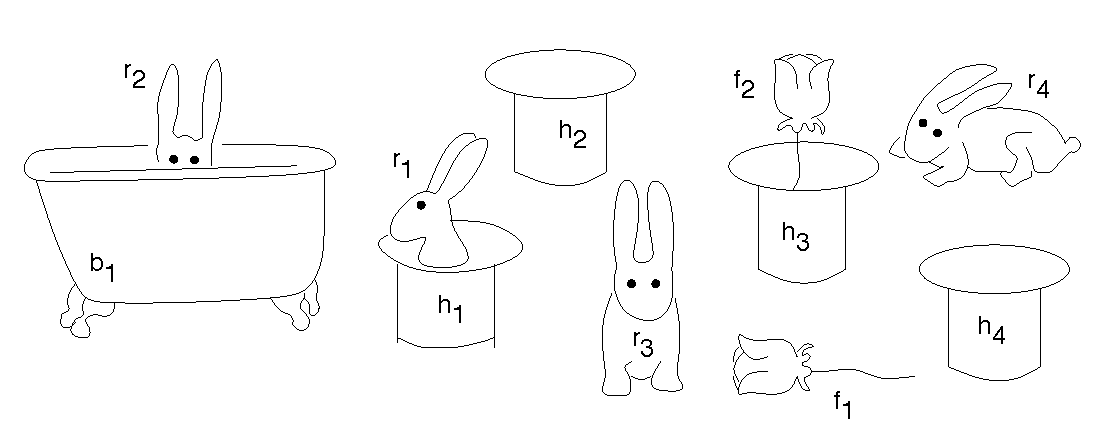
\includegraphics[width=\columnwidth]{pic-rabbits}
  \caption{``Take the rabbit from the hat'' (from \cite{Stone1998a}).}
  \label{fig:rabbits}
\end{figure}


\subsection{Coordinated referring expressions}

Consider the scene in Fig.~\ref{fig:rabbits}, and let's say we want to
instruct the hearer to remove the indicated rabbit, $r_1$, from the
indicated hat, $h_1$.  In the absence of further attributes that
distinguish $r_1$ from the other rabbits and $h_1$ from the other
hats, the best unique referring expression for $r_1$ is ``the rabbit
in the hat'' and the best unique RE for $h_1$ is ``the hat that
contains a rabbit''.  An NLG system which first computes the referring
expressions and then performs realization in a separate, subsequent
step would thus generate the sentence ``remove the rabbit in the hat
from the hat that contains a rabbit''.

\begin{figure}
  \centering
  
  \caption{A small SPUD-style lexicon.}
  \label{fig:spud-lexicon}
\end{figure}

\newcite{Stone1998a} showed that by coupling sentence planning and
realization more closely, the SPUD system is able to generate an
instruction that uses more succinct referring expressions: It is
sufficient to say ``remove the rabbit from the hat''.  There are two
aspects of SPUD that conspire to make this expression possible.
First, the lexicon entry for ``take X from Y'' in SPUD (shown in a
simplified version modelled after \newcite{KolSto07} in
Fig.~\ref{fig:spud-lexicon}) includes the ``semantic requirement''
that X must be in Y for the utterance to be felicitous.  Second, this
information is then used to coordinate the meanings of the two
referring expressions by means of a constraint network
\cite{dale91:_gener_refer_expres_invol_relat}.  In the example, the
semantic requirement of the verb would contribute the information
$in(x,y)$; the first NP would contribute the information $rabbit(x)$;
and the second NP would contribute $hat(y)$.  Taken together,
$\{in(x,y), rabbit(x), hat(y)\}$ is only satisfied by a single tuple
$(r_1,h_1)$, and therefore the reference is unique -- the two NPs can
restrict each other's extensions, mediated by the verb.


\subsection{A first planning approach}

Now let's talk about how this interaction between the two REs can be
modelled in a planning framework.  From the perspective of the
planning problem presented in Section~\ref{sec:gen-as-planning}, the
action instance for the verb's elementary tree instantiates the two
new REs with sets of distractors.  The purpose of each RE is then to
eliminate all distractors so a goal state can be reached.

\newcite{KolSto07} already go one step beyond what a pipelined model
could do by choosing all objects except for $r_1$ that are inside
something else (in the example, $\{r_2,f_2\}$) and all objects except
for $h_1$ that contains something ($\{h_3,b_1\}$) as the initial
distractor sets for the two NPs.  This exploits the semantic
requirement of the lexicon entry partially.  In this particular
example, it is not sufficient to generate ``the rabbit'' and ``the
hat'', because $r_2$ is also a rabbit and $h_3$ is also a hat.

However, this particular choice of distractor sets is not the only one
which, together with the information that X is in Y, would make the
joint reference unique.  For instance, if we can establish that the
first NP does not refer to $f_2$ and the second NP does not refer to
$b_1$, then we have again referred to $(r_1,h_1)$ uniquely.  More
generally, if we can find sets $A$ and $B$ such that 
$$\{(x,y) \mid x \notin A \;\mbox{and}\; y \notin B \;\mbox{and}\; in(x,y) \}
= \{(r_1,h_1)\},$$ 
then we will obtain a unique joint referring expression if we can
eliminate the distractors $A$ in the first NP and the distractors $B$
in the second NP.  The workload of establishing unique reference can
be shifted between $A$ and $B$: The more elements $A$ contains, the
more informative the first RE will have to be; but this will also
allow $B$ to be smaller, and so the second RE can be shorter.

Unfortunately, the computation of suitable sets $A$ and $B$ is beyond
the expressive power of a typical planning problem.  We can get around
this limitation by computing all possible (minimal) values for $A$ and
$B$ beforehand and encoding them in the planning problem.  To encode
the four minimal distractor sets for $r_1$ and $h_1$ in the example,
we can add the following conjunction to the initial state of the
planning problem:

$$
\begin{array}{l}
  \mathsf{distractorset}(s_1,\mathsf{in},r_1,h_1) \wedge
  \mathsf{distractor}_L(s_1,f_1) \wedge \\ \mathsf{distractor}_L(s_1,f_2)
  \wedge \mathsf{distractor}_L(s_1,r_3)  \wedge \\
%
  \mathsf{distractorset}(s_2,\mathsf{in},r_1,h_1) \wedge
  \mathsf{distractor}_L(s_2,f_2) \wedge \\ \mathsf{distractor}_R(s_2,h_3)
  \wedge \mathsf{distractor}_R(s_2,b_1) \wedge \\
%
  \mathsf{distractorset}(s_3,\mathsf{in},r_1,h_1) \wedge
  \mathsf{distractor}_L(s_3,f_1) \wedge \\ \mathsf{distractor}_L(s_3,f_2)
  \wedge \mathsf{distractor}_R(s_3,b_1) \wedge \\
%
  \mathsf{distractorset}(s_4,\mathsf{in},r_1,h_1) \wedge
  \mathsf{distractor}_L(s_4,r_3) \wedge \\ \mathsf{distractor}_L(s_4,f_2)
  \wedge \mathsf{distractor}_R(s_4,h_3) 
\end{array}
$$

These sets can then be picked up by the planning operators.  Operators
now receive an additional parameter for the choice of distractor sets,
and additional preconditions and effects as follows:

\action{S-takefrom-1}{u,x_1,x_2,x_3,s}
{\mathsf{distractorset}(s,\mathsf{in},x_2,x_3) \wedge \ldots}
{\forall y. \mathsf{distractor}_L(s,y) \rightarrow
  \mathsf{distractor}(\mathsf{pat}(u),y)
\wedge \\
\forall y. \mathsf{distractor}_R(s,y) \rightarrow
  \mathsf{distractor}(\mathsf{src}(u),y)
\wedge \ldots
}

We have implemented this conversion an evaluated the performance of
the FF planner \cite{HoffmannNebel01} on it.  FF is widely accepted as
an extremely efficient planner.  Unfortunately, it performs very
poorly on these examples.  For the above example, FF takes 22 seconds
to compute the sentence ``take the rabbit from the
hat''.\footnote{\todo{Measure runtimes on the same machine and say
    here what it is.}}  As the domain size increases, so does FF's
runtime: On a domain with four rabbits, four hats, three flowers, and
three bathtubs, plus random ``in'' relations between these, FF took
about 150 seconds on average.  For three rabbits and hats and four
flowers and bathtubs, FF ran out of memory before it was able to find
a plan.



%%% Local Variables: 
%%% mode: latex
%%% TeX-master: "rabbit-from-hat"
%%% End: 
